\documentclass[border=10pt]{standalone}

\usepackage{tikz}
\usepackage{tikzsymbols}
\usetikzlibrary{calc,patterns,shapes.geometric}

\def\centerarc[#1](#2)(#3:#4:#5){\draw[#1] ($(#2)+({#5*cos(#3)},{#5*sin(#3)})$) arc (#3:#4:#5);}

\begin{document}
	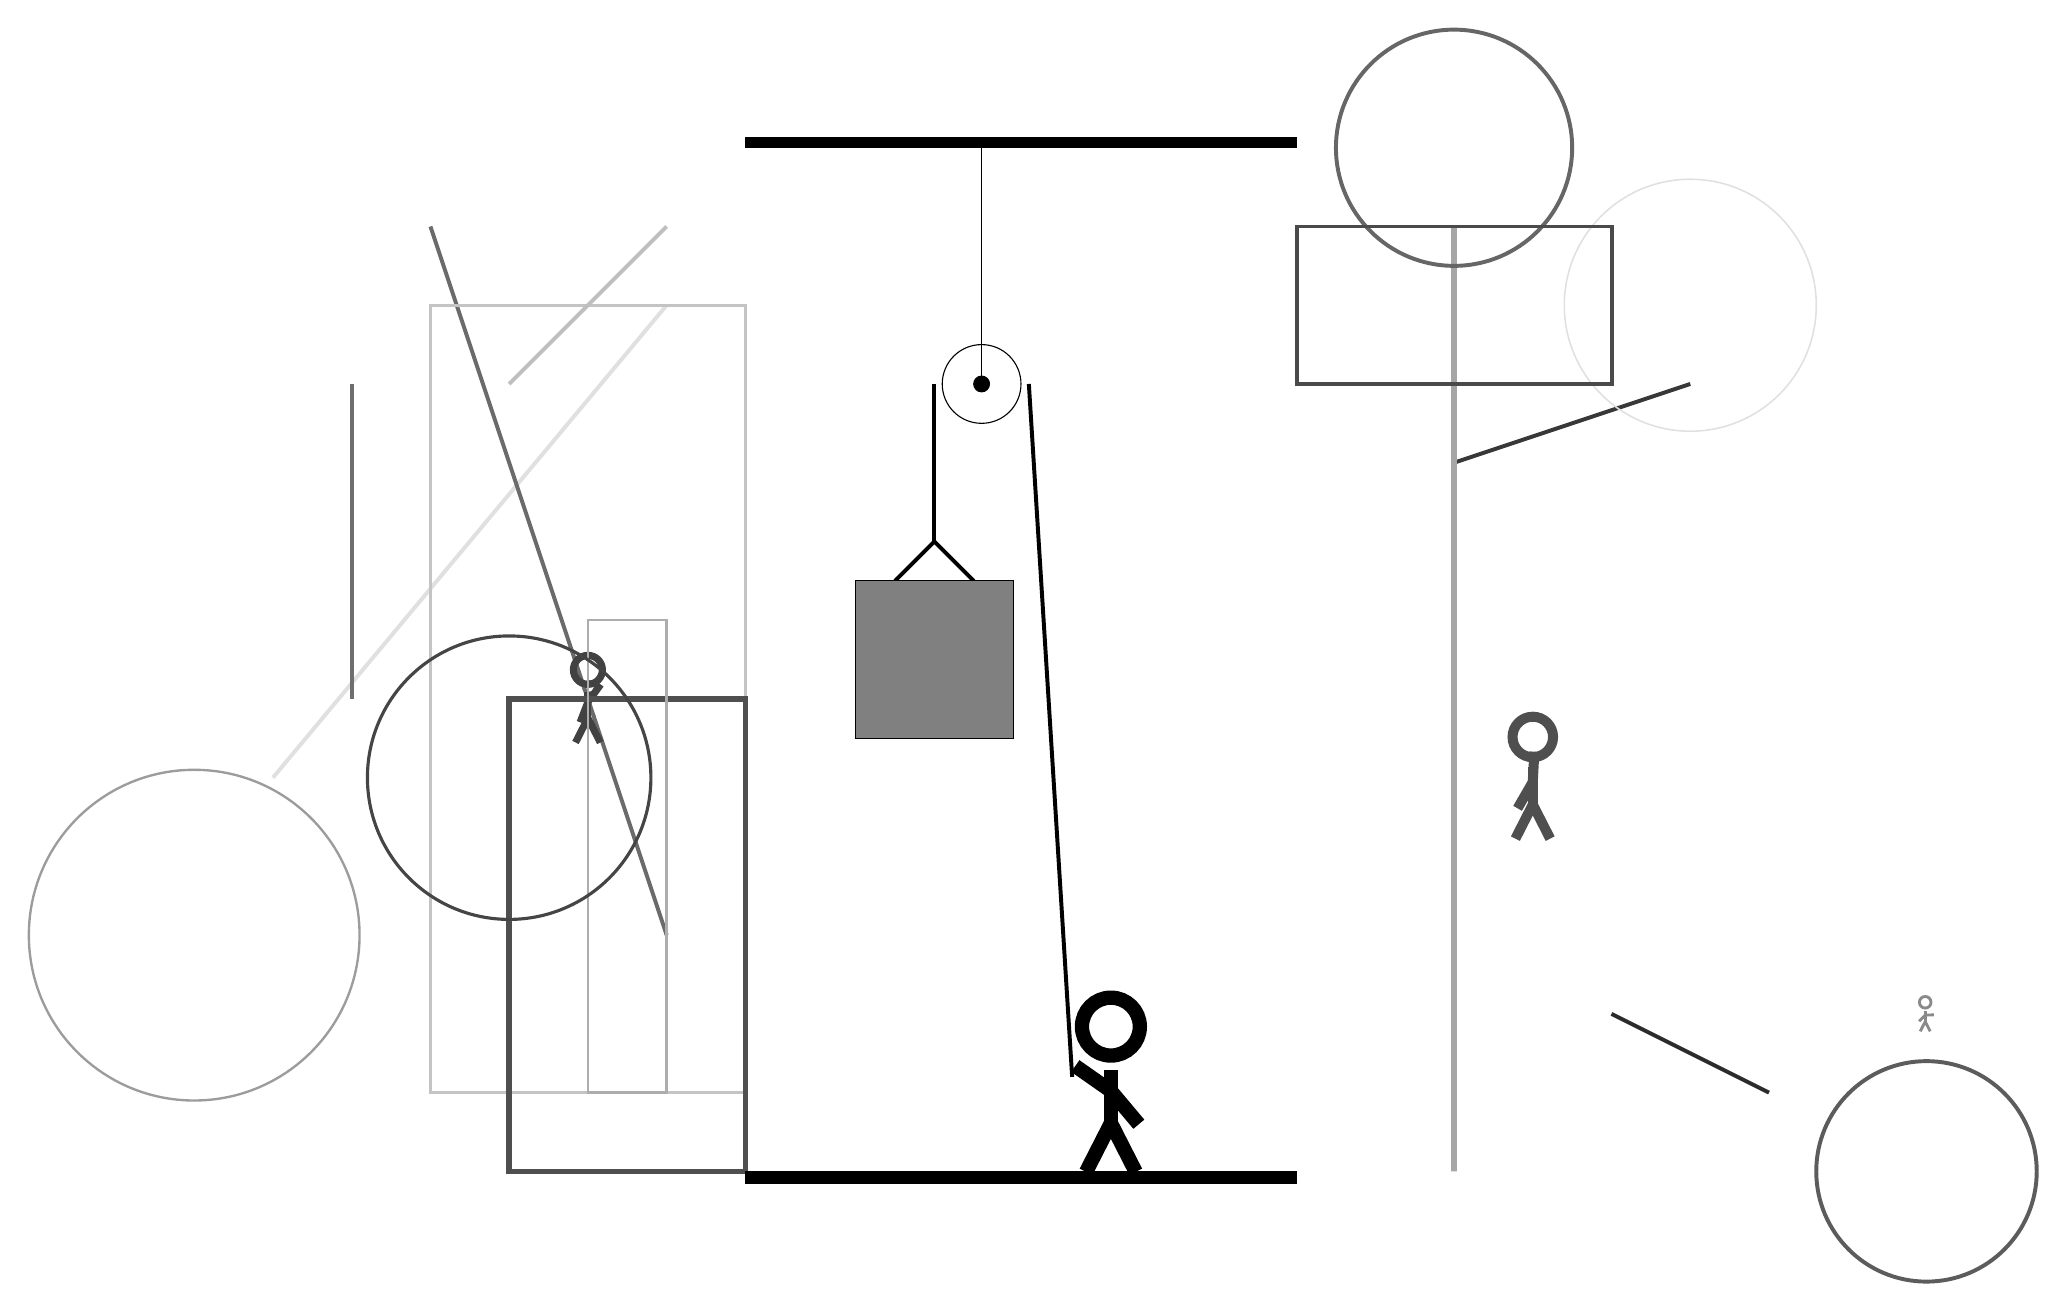
\begin{tikzpicture}
		%%%%% START %%%%%
		
		\draw[fill=black] (-2, 10) rectangle (5, 10.125);
		
		\draw (1, 7) circle (0.5);
		\draw[fill=black] (1, 7) circle (0.1);
		\draw (1, 10) -- (1, 7);
		
		\draw[line width=0.5mm] (-0.1, 4.5) -- (0.4, 5.0) -- (0.9, 4.5);
		\draw[fill=black!50] (-0.6, 4.5) rectangle (1.4, 2.5);
		
		\draw[line width=0.5mm, color=black!12](-3, 8) -- (-8, 2);
		
		\draw[line width=0.5mm, color=black!58](-3, 0) -- (-6, 9);
		\draw[line width=0.5mm, color=black!78](7, 6) -- (10, 7);
		\draw[line width=0.3mm, color=black!41] (7, 7) rectangle (7, 3);
		\draw[line width=0.4mm, color=black!23] (-2, 8) rectangle (-6, -2);
		\node[line width=0.7mm, color=black!58] at (-4, 3) {\Strichmaxerl[2][2][79]};
		\draw[line width=0.5mm, color=black!25](-3, 9) -- (-5, 7);
		\node[line width=0.5mm, color=black!46] at (13, -1) {\Strichmaxerl[2][45][2]};
		\node[line width=0.3mm, color=black!74] at (-4, 3) {\Strichmaxerl[5][69][54]};
		
		\draw [line width=0.3mm, color=black!39](-9, 0) circle (2.1);
		
		\draw[line width=0.5mm, color=black!57](-7, 7) -- (-7, 3);
		\draw[line width=0.7mm, color=black!35] (7, 9) rectangle (7, -3);
		\draw [line width=0.2mm, color=black!12](10, 8) circle (1.6);
		\draw[line width=0.5mm, color=black!83](9, -1) -- (11, -2);
		\draw [line width=0.5mm, color=black!64](13, -3) circle (1.4);
		\node[line width=0.5mm, color=black!69] at (8, 2) {\Strichmaxerl[7][60][87]};
		\draw[line width=0.7mm, color=black!69] (-2, 3) rectangle (-5, -3);
		
		\draw[line width=0.3mm, color=black!32] (-3, 4) rectangle (-4, -2);
		\draw [line width=0.5mm, color=black!60](7, 10) circle (1.5);
		\draw[line width=0.5mm, color=black!71] (5, 7) rectangle (9, 9);
		\draw [line width=0.4mm, color=black!73](-5, 2) circle (1.8);
		
		
		\draw[line width=0.5mm] (0.4, 7) -- (0.4, 5.0);
		\centerarc[line width=0.5mm](1, 7)(0:180:0.6);
		\draw[line width=0.5mm](1.6, 7) -- (2.15, -1.8);
		
		\node at (2.6, -1.9) {\Strichmaxerl[10][-35][-50]};
		
		\draw[fill=black] (-2, -3) rectangle (5, -3.15);
		
		%%%%% END %%%%%
	\end{tikzpicture}
\end{document}